\documentclass[aspectratio=169, xcolor=dvipsnames]{beamer}
\hypersetup{pdfpagemode=FullScreen}
\beamertemplatenavigationsymbolsempty
\setbeamertemplate{caption}{\raggedright\insertcaption\par}
\usepackage[utf8]{inputenc}
\usepackage[spanish]{babel}
\usepackage{siunitx}
\usepackage{graphicx}
\usepackage{xcolor}
\usepackage{amsmath}
\usepackage{esint}
\usepackage{biblatex}
\usepackage{multicol}
\usepackage{listings}
\usepackage{wrapfig}

\definecolor{myblue}{rgb}{0.29, 0.5, 0.94}
\definecolor{mygreen}{rgb}{0,0.6,0}

\lstdefinestyle{mystyle}{
    commentstyle=\color{mygreen},
    keywordstyle=\color{blue},
}
\lstset{style=mystyle}

\title{Aplicaciones de Sistemas Embebidos con Doble Núcleo}
\subtitle{Introducción a Sistemas Embebidos}
\author[Fabrizio Carlassara - Laboratorio de Sistemas Embebidos]{
\includegraphics[scale=0.15]{resources/images/utn_logo.png}}
\institute{UTN FRA\\Departamento de Ingeniería Electrónica\\Laboratorio de Sistemas Embebidos}
\date[]{\today} 
\usetheme{Warsaw}
\usecolortheme[named=myblue]{structure}
\setbeamertemplate{headline}{}

\begin{document}

\frame{\titlepage}
\begin{frame}{Introducción a Sistemas Embebidos}{Índice}
\begin{multicols}{2}
\tableofcontents
\end{multicols}
\end{frame}

\section{Sistemas Embebidos}
\subsection{Microcontroladores}
\begin{frame}{Introducción a Sistemas Embebidos}{Microcontroladores}
\begin{figure}
    \centering
    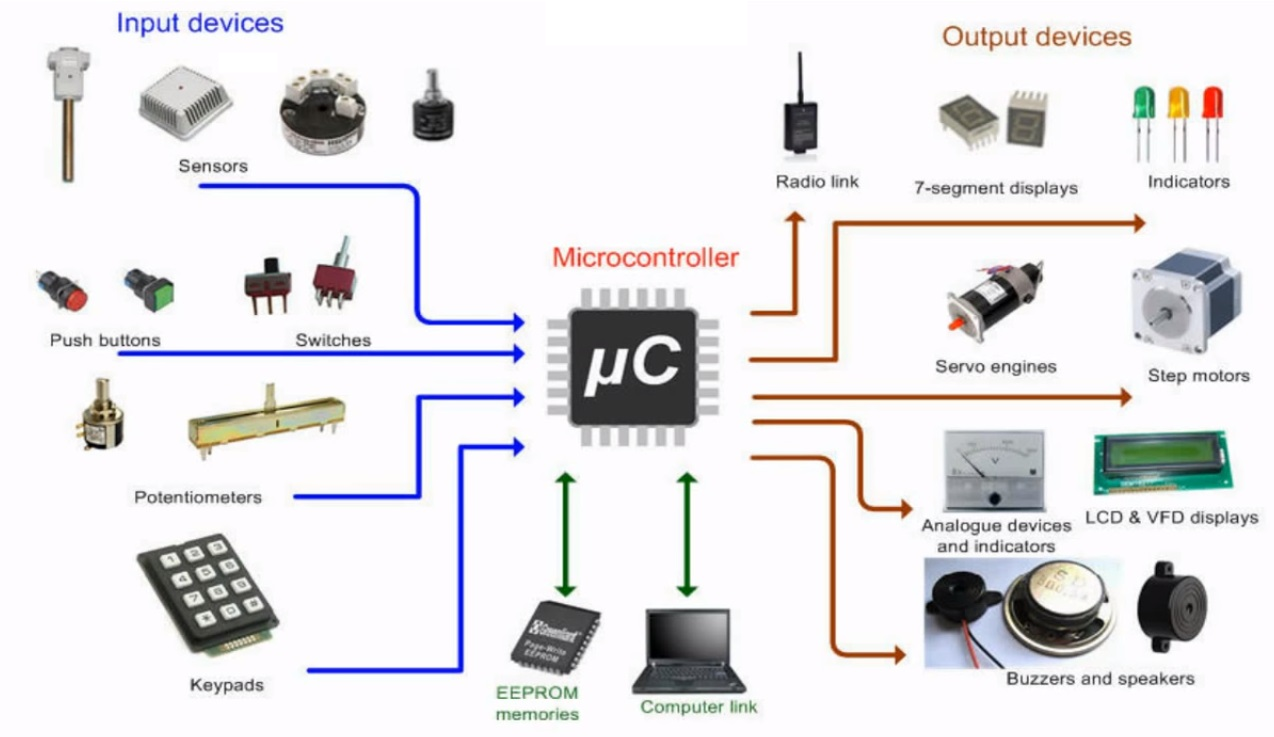
\includegraphics[width=0.8\linewidth]{resources/images/microcontroller.png}
\end{figure}
\end{frame}

\subsection{Aplicaciones}
\begin{frame}{Introducción a Sistemas Embebidos}{Aplicaciones}
    \begin{figure}
        \centering
        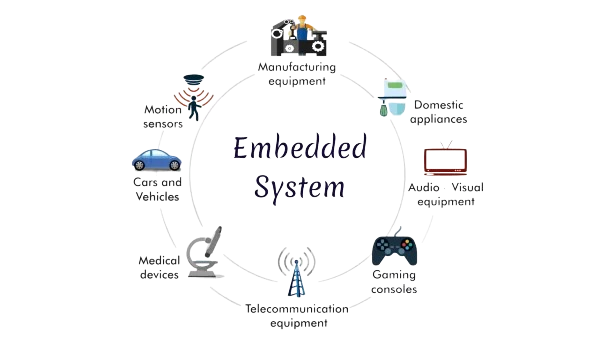
\includegraphics[width=0.8\linewidth]{resources/images/embedded_system.png}
    \end{figure}
\end{frame}

\section{ARM}
\subsection{Perfiles ARM}
\begin{frame}{Introducción a Sistemas Embebidos}{Perfiles ARM}
\begin{figure}
\begin{columns}
    \begin{column}{0.5\textwidth}
        \centering
        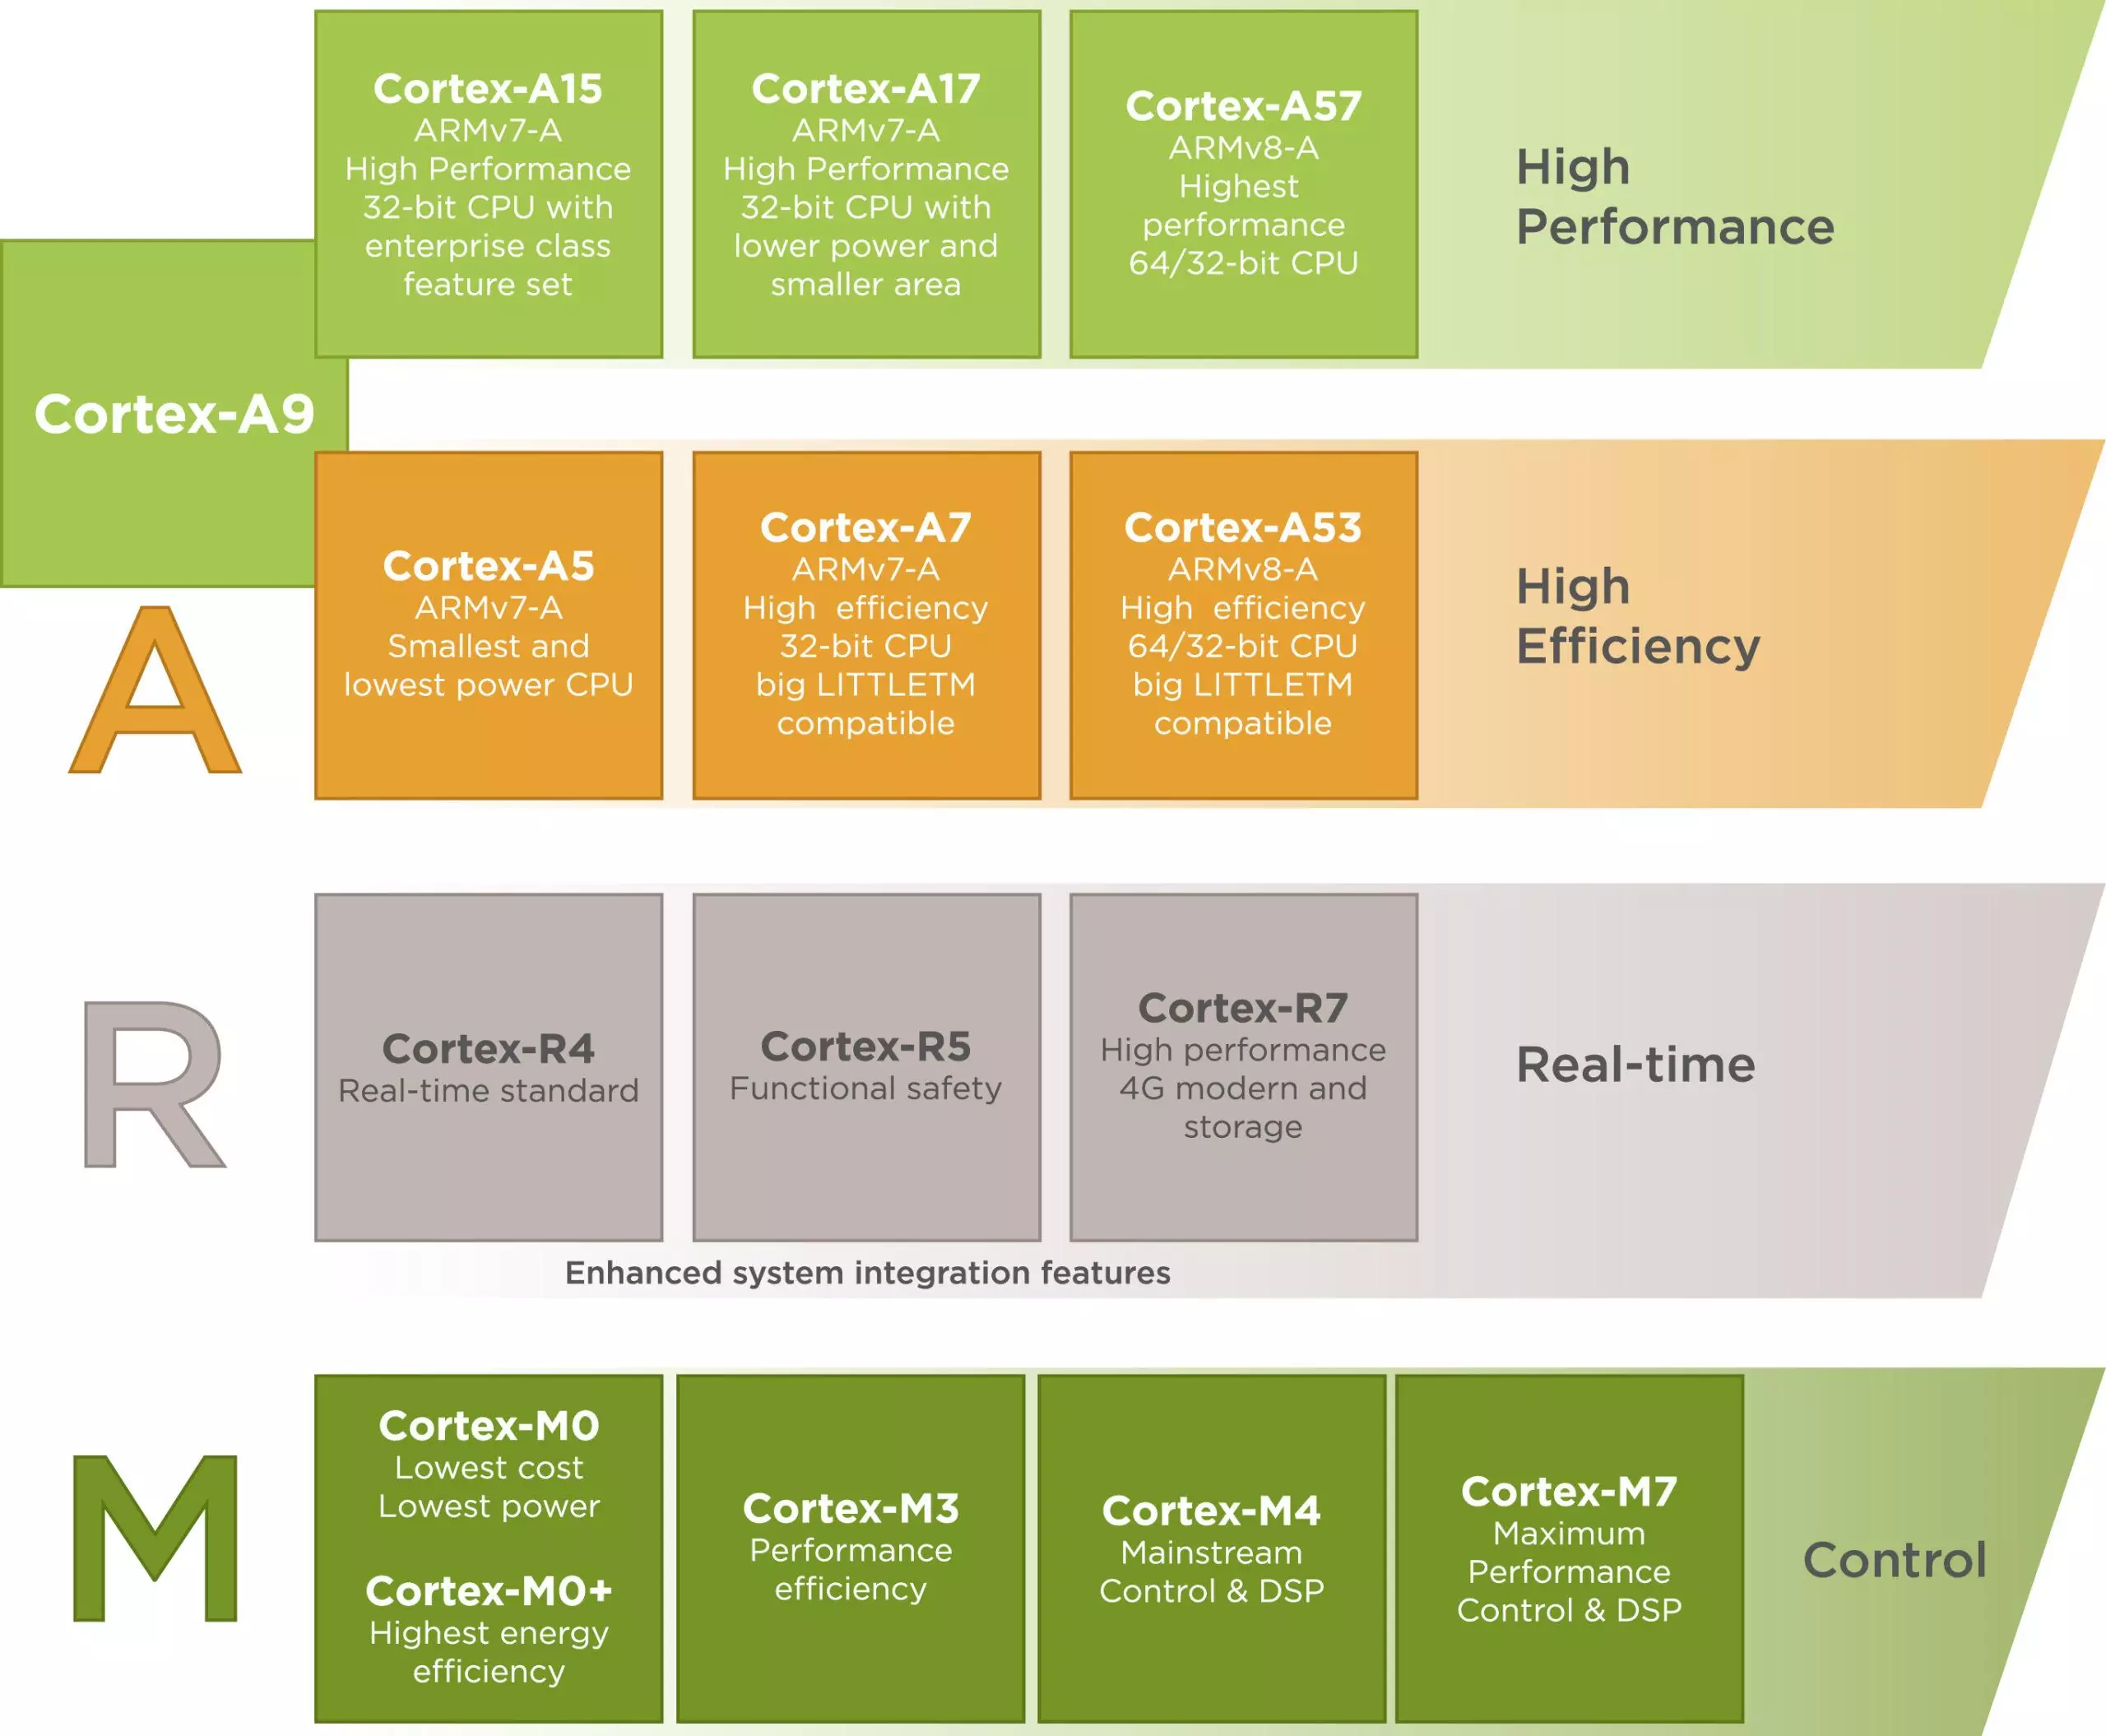
\includegraphics[width=0.8\linewidth]{resources/images/arm_profiles.png}
    \end{column}
    \begin{column}{0.5\textwidth}
        \begin{itemize}
            \item \textbf{Perfil A: Application}
                \begin{itemize}
                    \item Sistemas operativos de propósito general.
                    \item Aplicaciones de alta performance.
                \end{itemize}
            \item \textbf{Perfil R: Real-Time}
                \begin{itemize}
                    \item Aplicaciones de muy baja respuesta.
                \end{itemize}
            \item \textbf{Perfil M: Microcontroller}
                \begin{itemize}
                    \item Aplicaciones de muy bajo consumo.
                    \item Procesamiento de señales.
                    \item Aplicaciones específicas de bajos recursos.
                \end{itemize}
        \end{itemize}
    \end{column}
\end{columns}    
\end{figure}
\end{frame}

\subsection{Perfiles Cortex-M}
\begin{frame}{Introducción a Sistemas Embebidos}{Perfiles Cortex-M}
\begin{columns}
    \begin{column}{0.5\textwidth}
        \begin{itemize}
            \item \textbf{Cortex-M0/Cortex-M0+}
                \begin{itemize}
                    \item Más eficiente en consumo energético.
                    \item Mayoría de las aplicaciones comunes.
                \end{itemize}
            \item \textbf{Cortex-M3/Cortex-M4}
                \begin{itemize}
                    \item Unidad de punto flotante (FPU) e instrucciones de procesamiento de señales (DSP).
                \end{itemize}
            \item \textbf{Cortex-M7}
                \begin{itemize}
                    \item Máxima performance del perfil.
                    \item Aplicaciones de alta velocidad y recursos.
                \end{itemize}
        \end{itemize}
    \end{column}
    \begin{column}{0.5\textwidth}
        \begin{figure}
            \centering
            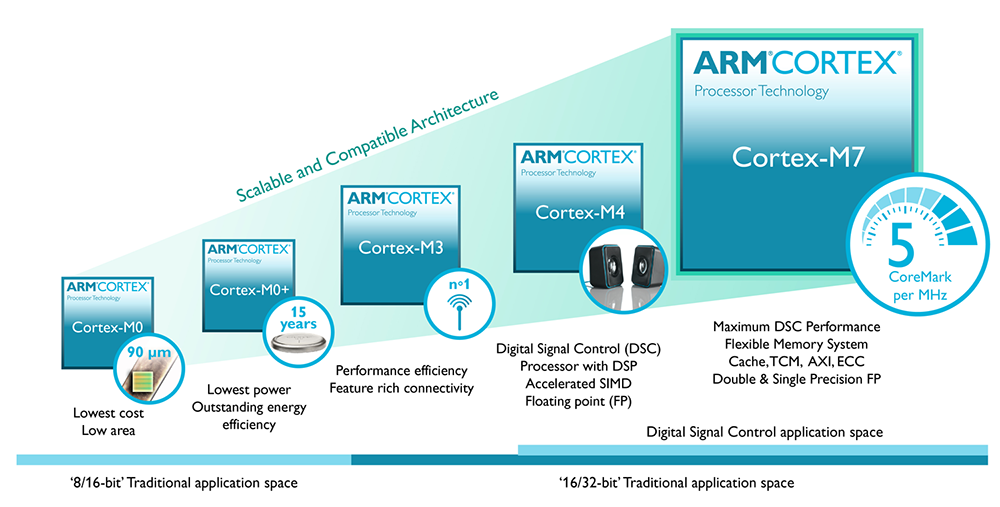
\includegraphics[width=0.85\linewidth]{resources/images/arm_cortex_m.png}
        \end{figure}
    \end{column}
\end{columns}
\end{frame}

\section{LPC845}
\begin{frame}{Introducción a Sistemas Embebidos}{LPC845 - Características}
\begin{columns}
\begin{column}{.5\textwidth}
    \begin{figure}
        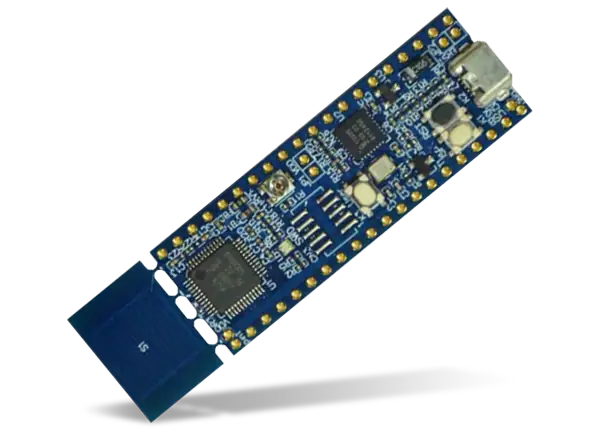
\includegraphics[width=0.75\linewidth]{resources/images/lpc845.png}
        \caption{LPC845 Breakout Board}
    \end{figure}
\end{column}
\begin{column}{.5\textwidth}
    Características principales
    \noindent\rule{\textwidth}{0.75pt}
    \begin{itemize}
        \item Cortex M0+ @ 30MHz
        \item 64KB Flash y 16KB RAM
        \item 54 GPIOs
        \item ADC 12 bits con 12 canales @ 1.2MS/s
        \item DAC 10 bits con 2 canales
        \item 4 I2C, 5 USART, 2 SPI
    \end{itemize}
\end{column}
\end{columns}
\end{frame}

\section{Git}
\subsection{Requerimientos}
\begin{frame}{Introducción a Sistemas Embebidos}{Git - Requerimientos}
\begin{columns}
\begin{column}{.65\textwidth}
    Requisitos para trabajar en el curso
    \noindent\rule{\textwidth}{0.75pt}
    \begin{itemize}
        \item Herramienta para manejo de Git (preferentemente Git por consola).
        \item Cuenta de GitHub personal.
        \item Forkear el \textcolor{myblue}{\href{https://github.com/utn-fra-lse/curso-lse}{repositorio del curso}}.
        \item Clonar localmente y traer los submódulos
        \begin{itemize}
            \item \textbf{git clone} para clonar el repositorio localmente.
            \item \textbf{git submodule init} para activar los submódulos.
            \item \textbf{git submodule update} para traer los submódulos.
        \end{itemize}
    \end{itemize}
\end{column}
\begin{column}{.35\textwidth}
\begin{figure}
    \centering
    \href{https://git-scm.com/}{
\includegraphics[width=0.2\linewidth]{resources/images/git_logo.png}}
    \caption{Git}
\end{figure}
\begin{figure}
    \centering
    \href{https://github.com}{
\includegraphics[width=0.2\linewidth]{resources/images/github_logo.png}}
    \caption{GitHub}
\end{figure}
\end{column}
\end{columns}
\end{frame}

\subsection{Workflow}
\begin{frame}{Introducción a Sistemas Embebidos}{Git - Workflow}
\begin{columns}
\begin{column}{.5\textwidth}
    Recuerden siempre!
    \noindent\rule{\textwidth}{0.75pt}
    \begin{itemize}
        \item \textbf{git add} para agregar cambios nuevos del directorio al staging area.
        \item \textbf{git commit} para pasar del staging area al repositorio local.
        \item \textbf{git push} para subir los cambios del repositorio local al repositorio remoto.
        \item \textbf{git pull --rebase} para traer cambios del repositorio remoto al local.
    \end{itemize}
\end{column}
\begin{column}{.5\textwidth}
\begin{figure}
    \centering
    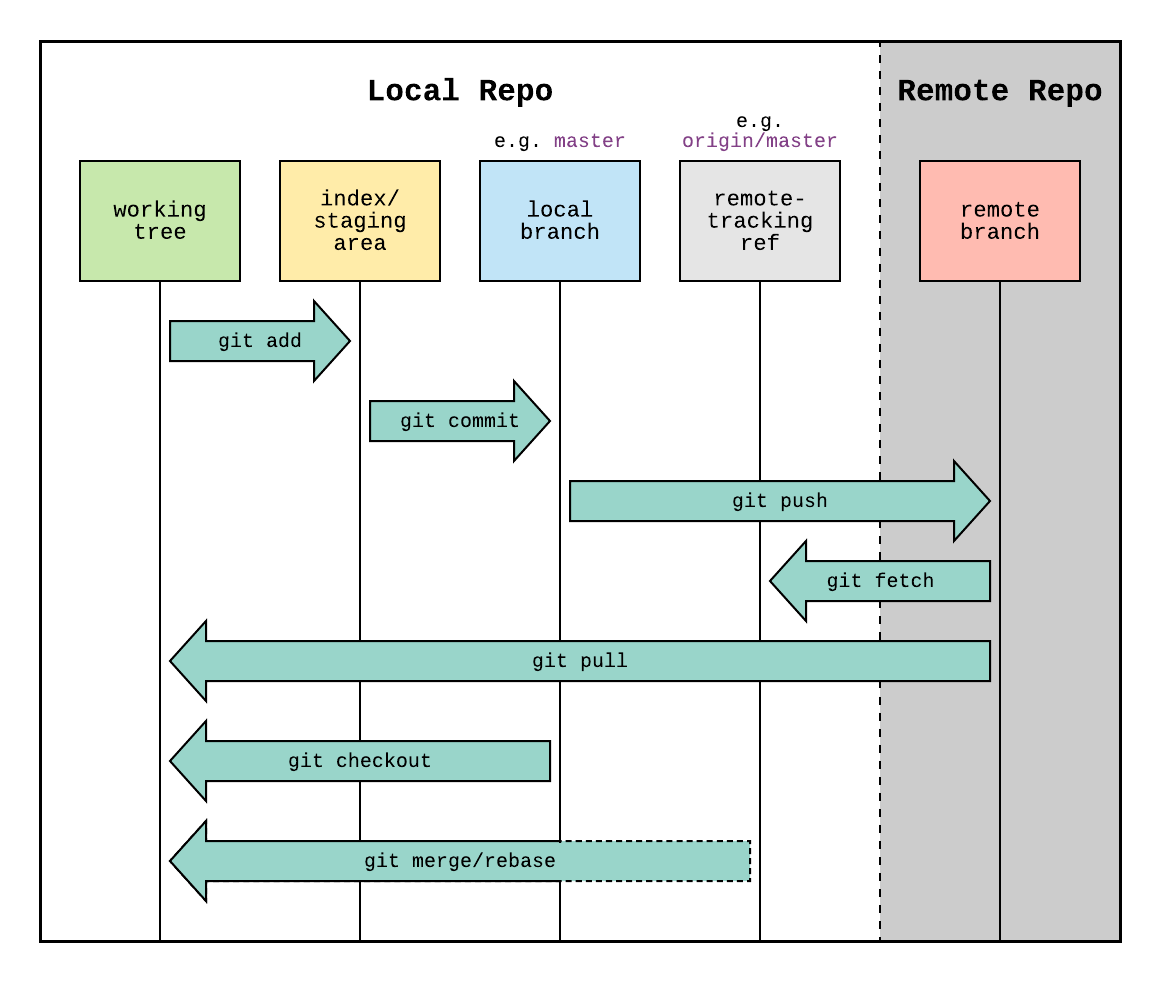
\includegraphics[width=0.9\linewidth]{resources/images/git_workflow.png}
    \caption{Flujo de trabajo de Git}
\end{figure}    
\end{column}
\end{columns}
\end{frame}

\section{MCUXpresso IDE}
\subsection{Crear un proyecto}
\begin{frame}{Introducción a Sistemas Embebidos}{Crear un proyecto}
\begin{columns}
\begin{column}{0.25\textwidth}
\begin{figure}
    \centering
    \href{https://www.nxp.com/design/design-center/software/development-software/mcuxpresso-software-and-tools-/mcuxpresso-integrated-development-environment-ide:MCUXpresso-IDE}{
\includegraphics[width=0.5\linewidth]{resources/images/mcuxpresso_ide.png}}
\end{figure}
\begin{figure}
    \centering
    
\includegraphics[width=0.5\linewidth]{resources/images/mcuxpresso_sdk.png}
\end{figure}
\end{column}
\begin{column}{0.75\textwidth}
    Crear un proyecto en MCUXpresso
    \noindent\rule{\textwidth}{0.75pt}
    \begin{itemize}
        \item Abrir el MCUXpreso y seleccionar de workspace el directorio workspace apropiado brindado por el repositorio del curso (lpc845/ejercicios).
        \item Al abrir el workspace, crear un nuevo proyecto para el LPC845 con:
            \begin{itemize}
                \item \textit{File / New / Create a new C/C++ Project...}
                \item \textit{SDK MCUs / LPC84x / LPC845 / lpc845breakout}
                \item \textit{LPC800 / LPC84x / C Project (Semihosted)}
                \item Asignar de nombre \textbf{01\_blinky}
                \item Continuar hasta crear el proyecto.
                \item En \textit{src/01\_blinky.c}, copiar este \href{https://github.com/utn-fra-lse/lpc845/blob/af536a2eef9075f1271c5c03d08e3999b701b55e/ejemplos/01_blinky/src/01_blinky.c}{ejemplo}.
            \end{itemize}
    \end{itemize}
\end{column}
\end{columns}
\end{frame}

\subsection{Depuración}
\begin{frame}{Introducción a Sistemas Embebidos}{Depuración}
Controles de depuración
\noindent\rule{\textwidth}{0.75pt}
\begin{columns}
\begin{column}{0.7\textwidth}
\begin{enumerate}
    \item Resume para que corra hasta el próximo breakpoint.
    \item Suspend para detenerlo en donde se encuentre actualmente.
    \item Terminate para terminar la depuración.
    \item Step Into entrar a la siguiente función.
    \item Step Over para correr la siguiente linea.
    \item Step Return para salir de la función actual.
    \item Restart para volver a comenzar el programa.
\end{enumerate}
\end{column}
\begin{column}{0.3\textwidth}
\begin{wrapfigure}{r}{1\textwidth}

\includegraphics[width=\linewidth]{resources/images/debug.png}
\caption{Controles para depurar}
\end{wrapfigure}
\end{column}
\end{columns}
\end{frame}

\section{Ejercicios}
\begin{frame}{Introducción a Sistemas Embebidos}{Ejercicios}
    Algunas propuestas para practicar
    \noindent\rule{\textwidth}{0.75pt}
    \begin{enumerate}
        \item En un proyecto llamado \textbf{01\_blinky}, hacer un programa en el que el LED Azul parpadee cada medio segundo aproximadamente.
        \item En un proyecto llamado \textbf{01\_antirebote}, hacer un programa que haga que el LED Rojo se prenda cuando se apriete el botón de USER y cuando se suelte se apague. Se debe implementar un antirebote por software en el botón.
        \item En un proyecto llamado \textbf{01\_animation}, hacer un programa que, mientras se apriete el botón de USER, se prenda de a uno los segmentos del display 7 segmentos (menos el G), formando una animación.
    \end{enumerate}
    \noindent\rule{\textwidth}{0.75pt}
    Cada ejercicio que se resuelva, subirlo al repositorio personal del curso.
\end{frame}

\section{Referencias}
\begin{frame}{Introducción a Sistemas Embebidos}{Referencias}
    Algunos recursos útiles
    \noindent\rule{\textwidth}{0.75pt}
    \begin{multicols}{2}
    \begin{itemize}
        \item \href{https://sirinsoftware.com/blog/the-arm-processor-a-r-and-m-categories-and-their-specifics}{Perfiles de ARM}
        \item \href{https://www.silabs.com/documents/public/white-papers/Which-ARM-Cortex-Core-Is-Right-for-Your-Application.pdf}{Aplicaciones para perfiles de ARM}
        \item \href{https://medium.com/@praveenmuth2/learn-how-git-works-internally-with-simple-diagrams-a9349dc32831}{Workflow de Git}
        \item \href{https://education.github.com/git-cheat-sheet-education.pdf}{Cheatsheet de Git}
        \item \href{https://community.nxp.com/pwmxy87654/attachments/pwmxy87654/mcuxpresso-ide/9289/1/MCUXpresso_IDE_User_Guide.pdf}{User Guide de MCUXpresso IDE}
        \item \href{https://github.com/utn-fra-lse/lpc845/blob/main/docs/UM11029.pdf}{Manual del LPC845}
        \item \href{https://github.com/utn-fra-lse/lpc845/blob/main/docs/UM11181.pdf}{Manual del LPC845 Breakout Board}
        \item \href{https://mcuxpresso.nxp.com/api_doc/dev/116/modules.html}{Documentación del SDK del LPC845}
        \item \href{https://www.nuvation.com/resources/article/switch-debouncing-electronic-product-designs}{Switch Debouncing for Electronic Product Designs}
        \item \href{https://github.com/utn-fra-lse/lpc845/blob/main/docs/BASE_KIT_V0.pdf}{Esquemático del kit del laboratorio}
    \end{itemize}
    \end{multicols}
\end{frame}

\end{document}
